\section{Introduction}

\subsection{Automatic Layout in GMF}
\begin{frame}
  \frametitle{Automatic Layout in GMF}
  \begin{itemize}
    \item GMF supports automatic layout...
  \end{itemize}
  \begin{center}
    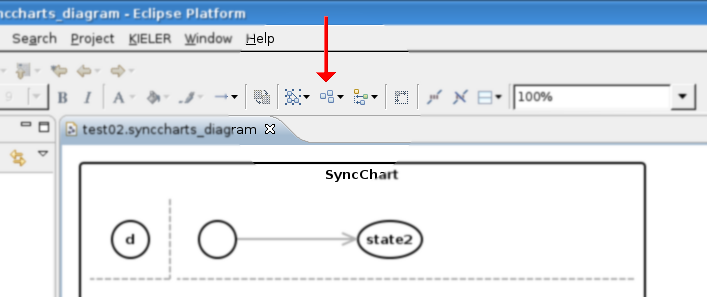
\includegraphics[width=0.8\textwidth]{images/gmf_layout.png}
  \end{center}
  \begin{itemize}
    \item<2> ...but is not very flexible
      \begin{itemize}
        \item No selection of different layout algorithms
        \item No customization of layout options
        \item No deep layout of compound structures
      \end{itemize}
  \end{itemize}
\end{frame}

\subsection{KIELER Meta Layout}
\begin{frame}
  \frametitle{KIELER Meta Layout}
  \begin{itemize}
    \item \alert{Meta} Layout: Allow fully flexible automatic diagram layout
      \begin{itemize}
        \item<2-> Contribute new layout algorithms using extension points
        \item<3-> Customize layout options in the properties view
        \item<4-> Layout compound structures recursively
        \item<5-> Layout different parts of a diagram with different
          options, or even with different layout algorithms
      \end{itemize}
    \item<6-> Development of special layout algorithms, e.g. for \alert{data
      flow diagrams}
  \end{itemize}
\end{frame}

\section{The Interface}

\subsection{Layout Providers}
\begin{frame}
  \frametitle{Layout Providers}
  Extension points are used to
  \begin{itemize}
    \item<1-> define diagram types
      \begin{itemize}
        \item {\small state machine, class diagram, etc.}
      \end{itemize}
    \item<2-> assign diagram types and layout options to specific parts of a GMF diagram
      \begin{itemize}
        \item {\small e.g. assign the ``class diagram'' type to the diagram edit part
          of a class diagram editor}
      \end{itemize}
    \item<3-> contribute new layout algorithms
      \begin{itemize}
        \item {\small call these contributions \alert{layout providers}}
      \end{itemize}
    \item<4-> define which diagram types are supported by the layout provider
    \item<5-> define new layout options and specify which options are understood
      by a layout provider
  \end{itemize}
\end{frame}

\subsection{Custom Layout Options}
\begin{frame}
  \frametitle{Custom Layout Options}
  \begin{itemize}
    \item To be implemented soon...
  \end{itemize}
\end{frame}

\subsection{Compound Structures}
\begin{frame}
  \frametitle{Compound Structures}
  \begin{itemize}
    \item Apply layout providers recursively
  \end{itemize}
  \begin{center}
    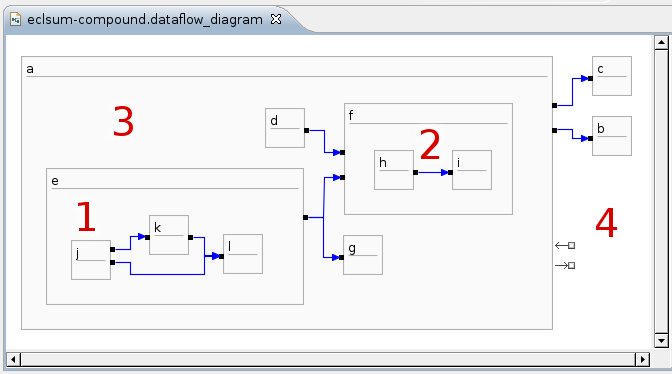
\includegraphics[width=0.9\textwidth]{images/compound-layout.png}
  \end{center}
\end{frame}

\subsection{Meta Layout}
\begin{frame}
  \frametitle{Meta Layout}
  \begin{center}
    {\Large Live Demo...}
  \end{center}
\end{frame}

\section{The Background}

\subsection{Diagram Layout}
\begin{frame}
  \frametitle{Diagram Layout}
  \begin{itemize}
    \item<1-> Layout providers work on an internal graph structure generated
      with EMF
    \item<2-> Need to map the contents of a diagram to the internal structure
      and back
    \item<3-> Done by \alert{Layout Managers} using the GEF command / request
      pattern
    \item<4-> Currently only a layout manager for GMF is implemented
      \begin{itemize}
        \item Analyzes the edit part structure at runtime
        \item Recursively go into the contents of an edit part to explore
          compound structures
      \end{itemize}
    \item<5-> Extension to other diagram editor generation frameworks is
      possible
  \end{itemize}
\end{frame}

\subsection{Data Flow Diagrams}
\begin{frame}
  \frametitle{Data Flow Diagrams}
  \begin{center}
    \includegraphics[width=0.8\textwidth]{kieler/simulink_dataflow01.pdf}
  \end{center}
  \begin{itemize}
    \item<1-> Operators exchange data through \alert{ports}
    \item<2-> Layout algorithms must respect these ports when routing connections
  \end{itemize}
\end{frame}

\begin{frame}
  \frametitle{Data Flow Diagrams: Special Algorithm}
  \begin{itemize}
    \item<1-> Developed a special algorithm to layout data flow diagrams
    \item<2-> Internal graph structure supports ports
    \item<3-> Integrated in the KIELER Meta Layout
    \item<4-> Also available as stand-alone library, successfully applied to
      \alert{Ptolemy}
  \end{itemize}
\end{frame}

\section*{}

\subsection{Summary}
\begin{frame}
  \frametitle{Summary}
    \begin{itemize}
    \item<1-> KIELER Meta Layout provides flexible automatic diagram layout
      \begin{itemize}
        \item Customize layout algorithms and layout options
      \end{itemize}
    \item<2-> Current implementation is able to layout all GMF diagrams
    \item<3-> Implemented a special layout algorithm for data flow diagrams
  \end{itemize}
\end{frame}
